\documentclass[aps,prl,preprint,showpacs,showkeys,linenumbers]{revtex4-1}
%\usepackage{hyperref}
\usepackage{graphicx}
\usepackage{tabularx}



\linespread{2}
\begin{document}
\title{Non-parabolicity and band gap re-normalisation in Si doped ZnO}
\author{R. E. Treharne}
\email[Corresponding Author: ]{R.Treharne@liverpool.ac.uk}
\affiliation{Stephenson Institute for Renewable Energy, University of Liverpool, UK}
\author{L. J. Phillips, K. Durose}
\affiliation{Stephenson Institute for Renewable Energy, University of Liverpool, UK}
\date{\today}
\begin{abstract}
\end{abstract}
\pacs{78.20.Jq, 88.66.sq, 81.15.-z}
\keywords{zinc oxide; magnetron sputtering; thin-film; doping; non-parabolicity, band gap normalisation}
\maketitle

\section{Introduction}



\section{Experimental Methods}

Films were deposited via RF magnetron sputtering using an AJA Phase II-J Orion system. The system was configured with a 'sputter-up' geometry with the substrate being suspended above two separate ceramic targets of ZnO and SiO$_2$ that were arranged off-centre and tilted at $5^{\circ}$ towards the middle of the substrate.  Soda-lime glass substrates (OptiWhite$^{TM}$, NSG) of size $100\times100\times4$ mm$^{3}$ were used throughout. They were cleaned by scrubbing with a nylon brush and a series of de-ionized water and isopropanol alcohol rinses followed by blow drying with a nitrogen gas jet. During deposition the ZnO and SiO$_2$ targets were sputtered from simultaneously using powers of $150$ W and $50$ W respectively. A growth pressure of 2mTorr Ar was used during deposition. The substrate temperature was maintained at $350\pm5^{\circ}$C during growth and the substrate was kept static (i.e was not rotated). Deliberate gradients of both thickness and composition were subsequently achieved across the resultant film to generate a `combinatorial' sample. A second film of pure SiO$_{2}$ was deposited under identical conditions (but without ZnO) to generate a reference film for calculating the \% wt. profile of SiO$_{2}$ in the co-sputtered film.

A Shimadzu UV-Vis-IR 3700 spectrophotometer with mapping capability was used to measure the transmittance of the co-sputtered film over the range 250 - 2500 nm. 289 spectra were taken in total at 5 mm increments over the full sample surface. At each of these 289 points the sheet resistance was also measured using a CMT-SR2000 4-point probe mapping system. Following transmittance and sheet resistance measurements the sample was cut into one hundred $10\times10$ mm$^2$ pieces. A selection of these pieces, 10 in total, were further scribed into four $5\times5$ mm$^2$ sections and Hall measurement were performed on each of these sections. The Hall measurement was performed with custom built equipment, provided by Semimetrics Ltd., using a field strength of 0.8 T.  Ellipsometry was performed on the same sections using a Woollam M2000-UI system. Ellipsometry was also used to map the thickness profile of the pure SiO$_{2}$ reference film.

\section{Results}\label{sec:2}

\subsection{Fitting of optical spectra}\label{sec:2.1}

Figure \ref{fig:1} shows a typical transmittance spectra taken from a single point on the combinatorial ZnO:Si sample. The full details of the model of the dielectric permittivity, $\varepsilon(\omega)$, used to fit the data are given in \cite{Treharne2012}. The key components of the model include: 1) a Lorentzian oscillator to account for the behaviour of the system's bound electrons and to provide a smoothly varying dielectric background over the range of interest ($250-2500$ nm), 2) an extended Drude model \cite{Mergel2002}, to characterise the system's free electron response, and 3) an inter-band transition model to account for the steep increase in the material's absorption coefficient ($\alpha \propto (E-E_G)^{1/2}$) in the vicinity of its direct band gap ($3.3 - 3.4$ eV). The two key parameters extractable from the dielectric model are the film's thickness, $d$, and plasma frequency, $\omega_{p}$, which is related directly to the carrier concentration according to
\begin{equation}
\label{eqn:1}
\omega_p = \sqrt{\frac{n_e e^2}{m_e \varepsilon_0}}
\end{equation}
where $m_e$ is the effective electrons (expressed in units of the free electron mass, $m_0$) and $\varepsilon_0$ is the permittivity of free space.

Fitting was achieved by using a Nelder-Mead downhill simplex algorithm \cite{Nelder1965}, implemented via python script, to minimize the quantity
\begin{equation}
\chi^{2} = \sum_{i}^N\sqrt{\frac{y_i - O_i}{N^2}}
\end{equation}\label{eqn:2}
where $N$ is the total number of data points in the spectra, $O_i$ the observed transmittance at each wavelength over the range of interest, and $y_i$ the theoretical transmittance calculated using the transfer matrix method \cite{Macleod1986} for a single thin-film on a finite, transparent substrate.  The fitting algorithm was iterated until the relative fractional change in consecutive $\chi^2$ values was less than $1\times10^{-6}$. The fitting of all 289 transmittance spectra taken over the combinatorial sample was fully automated, the only user input required being an initial estimate of film thickness at the point of the first spectrum. This automation ensured that the fitting of consecutive spectra was highly consistent. For all spectra, $\chi^2$ values of $<1$ were achieved indicating that all fits were as successful as that shown in figure \ref{fig:1}.

It was not possible to extract accurate values for the optical band-gap $E_G$ from the inter-band transition component of the model. All values were typically $\sim 0.2$ eV lower than expected (even once non-parabolicity and re-normalisation effects had been accounted for, see sections ~\ref{sec:2.2} and \ref{sec:2.3}).  This is due to the presence of a population of impurity states located in energy just below the bottom of the conduction band. The presence of these states generate a broadening, commonly referred to as an `Urbach tail' \cite{Urbach1953}, in the onset of the absorption coefficient. It is very difficult to determine the extent of this broadening by fitting the dielectric model to a single transmittance spectra. The use of variable angle spectroscopic ellipsometry (VASE) was therefore necessary to determine the true band gap of the material. 

For each point over the combinatorial sample surface a set of three ellipsometric spectra, taken at angles of 60, 65 and 70$^{\circ}$ with respect to a plane normal to the sample surface, was measured and fitted using a parameterized semi-conductor (PSEMI-M0) model \cite{Paulson1998} over the range $350 - 1000$ nm. The use of multiple spectra allowed the effect of the tail states to be extricated from the direct band to band transitions.  Figure \ref{fig:2} shows the difference in the $\alpha^2$ versus $E$ behaviour extracted from transmittance and ellipsometry data respectively. This disparity between band gaps extracted from the two techniques has been reported previously by Srikant \cite{Srikant1998}.

\subsection{ Conduction band non-parabolicity}
\label{sec:2.2}

For highly doped metal-oxides it has been shown that the conduction band, $E_c$, is `non-parabolic' and that the origin of this non-parabolicity may be attributed to a carrier dependent effective mass, $m_e(n_e)$. The functional form of this dependence, first suggested by Pisarkiewicz \textit{et. al} \cite{Pisarkiewicz1990}, is given by
\begin{equation}
\label{eqn:3}
m_e(n_e) = m_{e0}\sqrt{1+\frac{2C\hbar^2k}{m_{e0}}}
\end{equation}
where $m_{e0}$ is the value of the effective mass at the conduction band minimum and $C$ is the non-parabolicity factor, expressed in eV$^{-1}$. The carrier wave-number can be expressed in terms of the carrier concentration according to $k = (3\pi^2n_e)^{1/3}$. By re-examining equation \ref{eqn:1} it is clear that the relationship between $\omega_p^2$ and $n_e$ is becomes non-linear if the effective mass is not a constant. Figure \ref{fig:3} shows a plot of $\omega_{p}$, extracted from the spectrophotometry measurements, versus the carrier concentration, $n_e^H$, determined via Hall measurements, for the sample subset cut from the original combinatorial sample. A similar $\chi^2$ minimization procedure to that described in section \ref{sec:2.1}, in which the fitting parameters were $m_{e0}$ and $C$, was applied to the data set using
\begin{equation}\label{eqn:4}
\chi^2 = \sum_{i=1}^n\frac{(n_{e_i}^S-n_{e_i}^H)^2}{n^2}
\end{equation}
where the superscript $S$ corresponds to carrier concentrations calculated, using a carrier dependent effecitve mass $m_e(n_e)$ (equations ~(\ref{eqn:1}) a \ref{eqn:3}), from the spectroscopically determined plasma frequencies. The superscript $H$ denotes values of $n_e$ determined directly via Hall measurements. To determine the uncertainty associated with the fitted $m_{e0}$ and $C$ values a Monte-Carlo style error treatment \cite{Mendelsberg2009} was implemented within which the $\chi2$ minimization procedure was performed 1000 times. The inset plot in figure \ref{fig:3} shows the mean $m_e(n_e)$ relationship (solid line) and the corresponding spread (yellow line). An average extracted value of $m_{e0} = 0.35\pm0.02m_0$ is higher than previous published values of $0.24 - 0.28 m_0$ for the effective mass in undoped ZnO. An average extracted value of $C=0.30\pm0.01$ eV agrees very well with previously reported values of $\sim0.29$ ev$^{-1}$ \cite{Ruske2009, Ellmer2001} for Al doped ZnO films.

\subsection{ Band-gap renormalization}
\label{sec:2.3}

The optical band gap of a degenerately doped metal-oxide system increases as a function of carrier concentration (Burstein-Moss shift \cite{Burstein1954,Moss1954} according to
\begin{equation}
\label{eqn:5}
E_G = E_{G0} + \frac{\hbar^2(3\pi^2n_e)^{2/3}}{2m_{eff}}
\end{equation}
where$E_{G0}$ is the band-gap at the conduction band minimum and the joint density of states effective mass, $m_{eff}$ is given as
\begin{equation}
\label{eqn:6}
\frac{1}{m_{eff}} = \frac{1}{m_h}+\frac{1}{m_e(n_e)}
\end{equation}
A constant hole effective mass value of $m_h = 0.7m_0$ \cite{} is assumed throughout this work. Note that the non-parabolicity of the conduction band is accounted for when estimating the band gap by using the carrier dependent effective mass $m_e(n_e)$ determined in section \ref{sec:2.2}. The data points in figure \ref{fig:4} show the band-gap values, determined via ellipsometry, plotted against the Hall carrier concentrations. The points lie some distance from the relationship predicted by equation \ref{eqn:5}. The apparent reduction in the real band-gap values is due the re-normalization effects of many body electron-electron, electron-ion and hole-hole interactions. Lu \textit{et. al} \cite{Lu2007} have shown that the total energy shift due to re-normalization can be estimated by parameterising the detailed model described by $Jain$ \textit{et. al} according to 
\begin{equation}
\label{eqn:7}
E_R = An_e^{1/3} + Bn_e^{1/4} + Cn_e^{1/2}
\end{equation}
where $E_R$ is negative with respect to $E_G$. The $n_e^{1/3}$, $n_e^{1/4}$ and $n_e^{1/2}$ dependencies correspond to the exchange energy of free electrons, their correlation energy and the electron-ion interaction energy respectively. The coefficients $A$, $B$, and $C$, quantify the strength of each of these three dependencies. The coefficient values for the data shown in figure \ref{fig:4}, and a value for $E_{G0}$, was extracted using the established minimisation procedure. Table \ref{tab:1} show the extracted values and comparative values for n-type ZnO thin-films. The strength of the $n_e^{1/3}$ dependence is roughly three times than that reported for Al doped ZnO.

\section{Mapping of compositional dependence}
\label{sec:2.3}

Film thickness profiles were determined for the combinatorial ZnO:Si and SiO$_{2}$ samples. The $\%$ wt. SiO$_{2}$ content at each point over the combinatorial sample was estimated according to
\begin{equation}
\label{eqn:8}
x = \frac{\Gamma_{B}d_{B}}{\Gamma_Ad_A+\Gamma_{B}d_{B}}\times100\%
\end{equation}
where $\Gamma_A$ and $\Gamma_B$ are the bulk densities of ZnO and SiO$_{2}$ respectively and $d_A$ and $d_B$ are the corresponding thicknesses, $d$, of the ZnO and SiO$_{2}$ films. The carrier concentration profile for the combinatorial sample was calculated from extracted $\omega_p^S$ values according to equation \ref{eqn:1} and using the non-parabolic effective mass relationship, $m_e(n_e)$, determined in section \ref{sec:2.2}. The corresponding mobility profile was calculated according to
\begin{equation}
\label{eqn:9}
\mu_e=\frac{1}{n_e^SR_Sde}
\end{equation}
where $R_S$ are the sheet resistance values obtained directly from 4 point probe measurements. Figure \ref{fig:3} shows the three dimensional contour profiles of $n_e$ and $\mu_e$ accross the surface of the combinatorial sample. In both cases, a maximal ridge, corresponding to $n_e\sim 4.5$ cm$^{-3}$ an $\mu_e \sim 16$ cm$^2$V$^{-1}$s$^{-1}$, runs diagonally across the sample. By superimposing the contour distribution of $\%$ wt. SiO$_{2}$ content (dotted black contour lines) a very strong correlation between carrier concentration and composition becomes apparent, the maximum $n_e$ and $\mu_e$ values corresponding to a value of $x=0.65\%$ wt. SiO$_{2}$ content.

By plotting the distributions of $n_e$ and $\mu_e$ with respect to $x$ the compositional dependence can be observed directly, see figure \ref{fig:4}. Here the strength of the combinatorial analysis is fully appreciated by its ability to generate continuous, non-ambiguous distributions of the material's electrical behaviour and shows that it is highly sensitive to the composition - the resistivity spanning over three orders of magnitude within the compositional range $x = 0 - 0.65\%$ wt. SiO$_{2}$. Furthermore, the uncertainty in the optimum value of $x$, that minimises the resistivity, is significantly reduced when compared to the multi-sample analyses that are commonly reported. 

The solid straight line in the $n_e$ vs $x$ plot indicates the relationship predicted for  a $100\%$ doping efficiency, i.e. where every Si atom incorporated into film substitutionally replace a Zn atom and contributes two free electrons to the system. For low values of $x$, i.e. in the range $0 - 0.5\%$ wt. SiO$_{2}$, this relationship is adhered to. However as $x$ increases further the doping efficiency decreases rapidly and the carrier concentration is limited to $3-4\times10$ cm$^{-3}$ for compositions up to $10\%$ wt. SiO$_{2}$. After the optimum value of $x$ is reached the mobility drops off steeply and approaches a value of zero for values of $x$ beyond $6\%$. This suggests that as $x$ is increased beyond the optimum composition, Si is no longer incorporated into the film as a substitutional dopant and instead acts to increase the scattering of the free carriers, existing as an interstitial impurities or forming segregated Si-O phases at the grain boundaries. 



\subsection{Scattering}
\label{sec:2.4}

The behaviour of carrier mobility can be described further by considering its direct relationship with the carrier concentration. Figure \ref{fig:5} shows that by plotting $\mu_e$ versus $n_e$ for all data points two distinct populations are revealed. The red data points correspond to compositions $x<0.65\%$. Within this distribution, and for carrier concentrations below $2.5\times10$ cm$^{-3}$ the mobility of the free carriers can be described in terms of a grain barrier limited transport  model proposed by  Seto $et. al$ \cite{Seto1975}. The model assumes that at the grain boundaries a population of filled trap states exist within the band gap. This causes the conduction band to bend upwards at each grain boundary forming a barrier to charge transport. The inter-grain mobility, $\mu_B$ of free carriers is therefore limited by thermal processes according to 
\begin{equation}
\label{eqn:10}
\mu_{ig} = \mu_0\exp(-\frac{\Phi_B}{k_BT})
\end{equation}
where $\Phi_B$ is the barrier height at the grain boundary and is related directly to the carrier concentration according to
\begin{equation}
\label{eqn:11}
\Phi_B=\frac{e^2n_t}{8\varepsilon_{\infty}\varepsilon_0n_e}
\end{equation}
where $n_t$ is the trap density and $\varepsilon_{\infty}$ is the high frequency dielectric permittivity ($\varepsilon_{\infty}\sim8.3$ for single crystal ZnO \cite{Ashkenov2003}). The pre-factor $\mu_0$ is the internal mobility of the grain, expressed as
\begin{equation}
\label{eqn:12}
\mu_0=\frac{eL}{\sqrt{2\pi m_ek_BT}}
\end{equation}
where $L$ is the grain size. It is necessary to extend the Seto model in the case of degenerately doped ZnO to account for the tunnelling of carriers through the barrier $\Phi_B$. As the carrier concentration increases the Fermi level rises towards the top of the barrier while the barrier height decreases proportionally to $1/n_e$. Following the onset of tunnelling the effective carrier mobility increases exponentially with respect to carrier concentration. The mobility and is eventually limited by other scattering processes, for example ionized-impurity scattering. A semi-empirical relationship the mobility due to the tunnelling of free carriers , $\mu_t$ can be expressed according to
\begin{equation}
\label{eqn:13}
\mu_t = \frac{\mu_{ii}-\mu_{ig}}{1+\exp[-\frac{1}{\alpha}(\Delta_{BM}+E_R-\beta\Phi_B)}
\end{equation}
where the factor $\alpha$ accounts for the sharpness of the onset in tunnelling and is likely to be related to the depletion width of the grain boundary. A second empirical factor, $\beta$ takes into account of any extra functional dependence of $\Phi_B$ on $n_t$ which is likely vary with respect to $n_e$. The effective mobility may therefore be expressed as the sum of the inter-grain and tunnel mobilities according to
\begin{equation}
\label{eqn:14}
\mu_{eff} = \mu_{ig}+\mu_{t}
\end{equation}
Figure \ref{fig:5} shows corresponding the fit of this extended model to the data in the region of composition $x<0.65\%$. An extracted value of $n_t = 1.79\times10^{14}$ cm$^{-3}$ is over two orders of magnitude greater than that reported for reactively sputtered, undoped ZnO films \cite{Carcia2003} and an order of magnitude greater than that for Al doped ZnO films \cite{Shigesato2003}. This is reflected in the relatively low optimum mobility values of $\sim16$ cm$^{2}$V$^{-1}$s$^{-1}$ which is typically half that of Al doped ZnO films. The reduction of the level trap densities at the grain boundaries is therefore key to the improvement of carrier mobility in Si doped ZnO films. This is likely to be achieved through further investigations of the effect of growth parameters, i.e. substrate temperature and sputter pressure. Based on the model used in this work, a reduction of $n_t$ by $sim20\$$ could yield a doubling of the mobility.

The green data points in figure \ref{fig:5} show the $n_e$ versus $\mu_e$ behaviour for $>0.65\%$ wt. SiO$_2$ compositions. The mobility now tends towards a minimum value at a higher carrier concentration of $\sim 3$ cm$^{2}$V$^{-1}$s$^{-1}$. This is indicative of an increased trap density, the result of an excess of Si at the grain boundaries or perhaps the formation of Si-O phases.  

\section{Conclusions}
\label{sec:4}
A consideration of the non-parabolicity of the conduction band for Si doped ZnO has yeilded estimates for the values of the band minimum effective mass, $m_{e0} =0.35m_0$, and the non-parabolicity factor, $C=0.3$ eV$^{-1}$. The non-parabolicity contributes to a reduction in the expected Burstein-Moss shift of the optical band-gap at carrier concentrations beyond $10^{20}$ cm$^{-3}$. Further reductions in the band-gap arises from the renormalization effects which are dominated by electron-electron and electron-ion interactions. For Si doped films the component of the magnitude of these effects are significantly greater than that reported for sputtered Al doped ZnO films.

The combinatorial methodology employed within this work allows the relationship between composition and the electrical behaviour to be determined with excellent accuracy, with a continuous distributions between $n_e$, $\mu_e$, $\rho$ and $\%$ wt. SiO$_{2}$ being determined. Furthermore, the extraction of all data from a single sample ensures that a high level of consistency between each data point is achieved compared with measurements taken over a series of separately deposited samples. Maximum values of $4.5\times10^{20}$ cm$^{-3}$ and $16$ cm$^{2}$V$^{-1}$s$^{-1}$ were achieved for the carrier concentration and mobility respectively, at an optimial composition of $x =0.65\%$ wt. SiO$_2$, and this corresponding to a minimum resistivity of $8.7$ $\Omega$.cm.

The model of grain boundary scattering proposed by $Seto$ \cite{Seto1975} has been extended to include the effects of tunneling through grain boundaries. The model generates a good agreement for the observed $\mu_e$ versus $n_e$ behavious at compositions up to the optimum value of $x$. The model highlights a potential route to improving carrier mobility, i.e. by reducing the density of trap states that exist at the grain boundaries.

Above the optimum composition a different dependence is observed to that below it. This is thought to be due to the increased density of trap states associated with the incorporation of excess Si into the films.
\begin{acknowledgements}

\end{acknowledgements}

\bibliography{ref}


\begin{figure}[0]
\centering
\caption{\label{fig:1}}
\end{figure}

\begin{figure}[p]
\centering
\caption{\label{fig:2}}
\end{figure}

\begin{figure}[p]
\centering
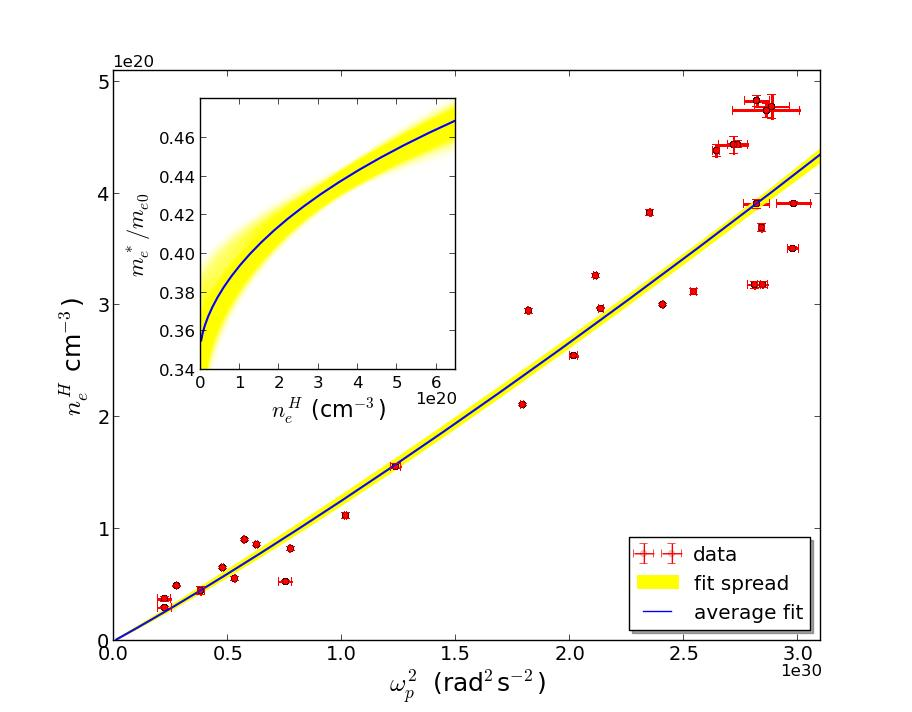
\includegraphics[width = 0.8\textwidth]{figure1c}
\caption{\label{fig:3}}
\end{figure}

\begin{figure}[p]
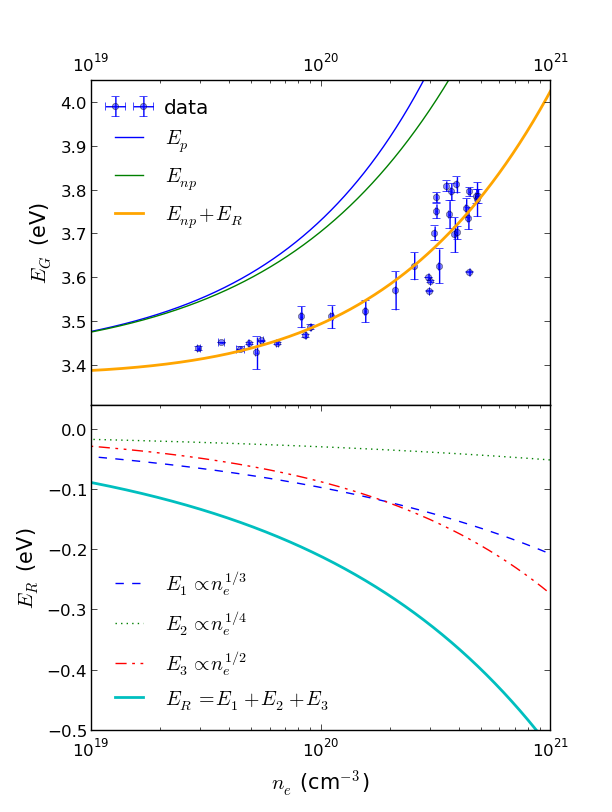
\includegraphics[scale=0.8]{figure5_b.png}
\caption{\label{fig:4}}
\end{figure}


\begin{figure}[p]
\centering
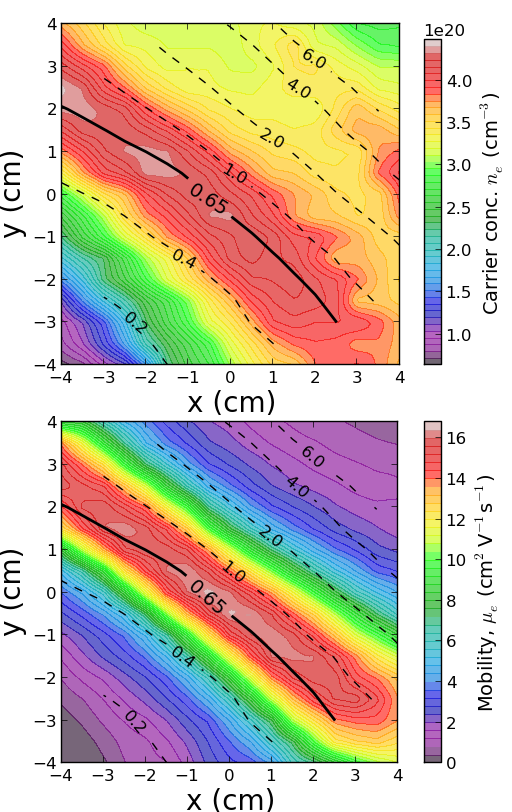
\includegraphics[scale=0.8]{figure2.png}
\caption{\label{fig:5} Contour maps of carrier concentration and mobility over the combinatorial sample. The (--) contour lines show an overlay of the \% wt. SiO$_{2}$ composition.}
\end{figure}

\begin{figure}[p]
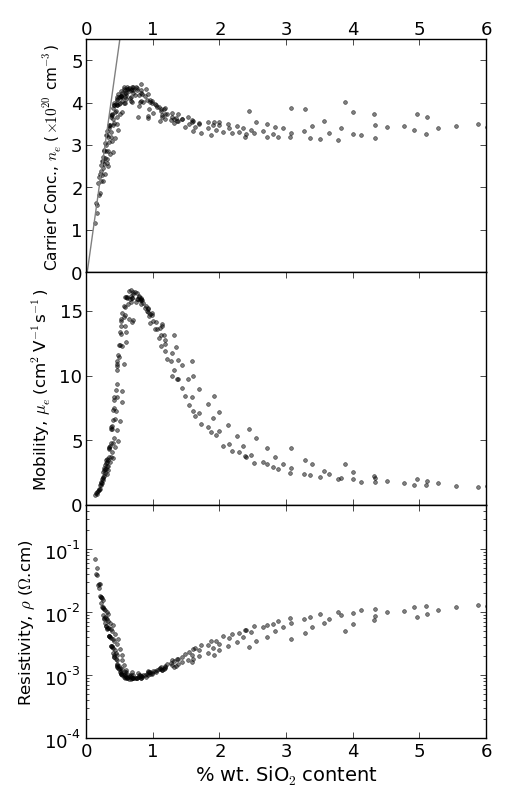
\includegraphics[scale = 0.85]{figure3.png}
\caption{\label{fig:6} Distributions of carrier concentration, mobility and resistivity with respect to \% wt. SiO$_{2}$ content. The maximum values for $n_e$ ($4.4\times10^{20}$ cm$^{-3}$) and $\mu_{e}$ ($16.5$ cm$^{2}$V$^{-1}$s$^{-1}$) coincide with a composition of $0.65$\% wt. SiO$_{2}$. The solid straight line in the top plot shows the maximum theoretical carrier concentration with respect to SiO$_{2}$ content should every incorporated Si atom be substituted at a Zinc site and donate 2 carriers.}
\end{figure}

\begin{figure}[p]
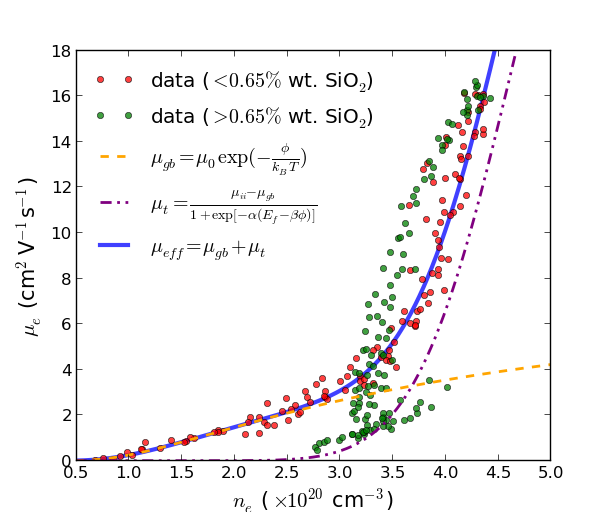
\includegraphics[width=1\textwidth]{figure4.png}
\caption{\label{fig:7} }
\end{figure}


\begin{table}[p]

\centering
\begin{tabularx}{0.7\textwidth}{ >{\setlength\hsize{1\hsize}\raggedright}X>{\setlength\hsize{1\hsize}\centering}X@{} >{\setlength\hsize{1\hsize}\centering}X }
  \hline\hline
Parameter 1 & Extracted Value & Copmparison \cite{Lu2007} \tabularnewline
\hline
$A$ ($\times10^{-8}$ eV.cm)  & $2.1\pm0.8$  & 0.69 \tabularnewline
$B$ ($\times10^{-7}$ eV.cm$^{3/2}$) & $3.0\pm2.6$  &  1.6 \tabularnewline
$C$ ($\times10^{-7}$ eV.cm$^{3/4}$) &  $8.7\pm1.5$  & 7.76 \tabularnewline
$E_{G0}$ (eV) & $3.41\pm0.01$ & - \tabularnewline
\hline\hline
\end{tabularx}
\caption{\label{tab:1} This is the caption}
\end{table}



\end{document}